\section{Resultados}
% Deben incluir los resultados de los experimentos, utilizando el formato mas
% adecuado para su presentacion. Deberan especicar claramente a que
% experiencia corresponde cada resultado. No se incluiran aqu corridas de
% maquina. Algo fundamental en su aprendizaje en la materia es la presentacion
% de resultados de forma clara y concisa para el lector

\subsection{Hipótesis}
Como vimos en la Introducción Teórica, Newton tiene convergencia cuadrática y Secante $supralineal$ (alrededor de 1.6).\\

Sería normal suponer que Newton tiene mejor performance dado que converge más rápido. Sin embargo para comparar performance, debemos considerar costo como rapidez de convergencia. Un algoritmo que converge rápido pero tarda algunos segundos por iteración podría tomar mas tiempo que uno que converge mas lento pero toma solo algunos milisegundos por iteración.\\

Podemos asumir que el costo de una iteración está marcado por la evaluación de la función, de hecho, este vendría a ser nuestro caso. Entonces la cantidad de evaluaciones de una función puede ser una buena medida de costo.\\

Secante solo requiere una evaluación de la función por iteración, dado que el valor de $f(x_{n - 1})$ se puede guardar de la iteración previa.\\

Newton requiere una evaluación de la función y otra de su derivada por iteración. Es complicado estimar el costo de evaluar la derivada en general. En algunos casos la derivada puede ser fácil de evaluar y en otros puede ser incluso mas difícil de evaluar que la función original.\\

Podemos asumir entonces, que en general, calcular la derivada es al menos tan costoso como calcular la función. Por lo tanto asumimos que Newton va a tomar dos evaluaciones por iteración.\\

Este análisis nos lleva a suponer que Secante debería ser mas performante que Newton en general.

\subsection{Casos de Prueba}
La aproximación inicial que tuvimos fue tomar cada uno de los parámetros, fijar los demás y hacer un análisis de cada uno de los factores de estudio (tiempo, iteraciones, convergencia, etc.) haciendo crecer los parámetros de turno. Claramente la cantidad de casos era mucha y en general los resultados eran difíciles de interpretar y no aportaban al propósito de develar si nuestra hipótesis se cumplía.\\

Por lo tanto decidimos que lo mejor sería solamente tomar un par de combinaciones de todas las posibles que nos parecieran que fueran representativas. En nuestro caso al ya tener $x_0$ y $x_1$ definidos en base a previa experimentación decidimos hacer comparaciones entre los métodos en términos de iteraciones y tiempo de ejecución para $\alpha$'s crecientes.\\

\subsubsection{Iteraciones} % (fold)
\label{ssub:iteraciones}

En el caso de hacer crecer $\alpha$ para ver cómo se comportan en función de las iteraciones, nuestra suposición es que Newton tomará menos iteraciones que Secante. Ahora, para Newton con $f(x)$ y $e(x)$ suponemos que el primero tomará menos iteraciones ya que el segundo cuenta con un cociente extra para calcular con respecto al primero en cada iteración.\\

\begin{figure}[!htbp]
  \begin{center}
    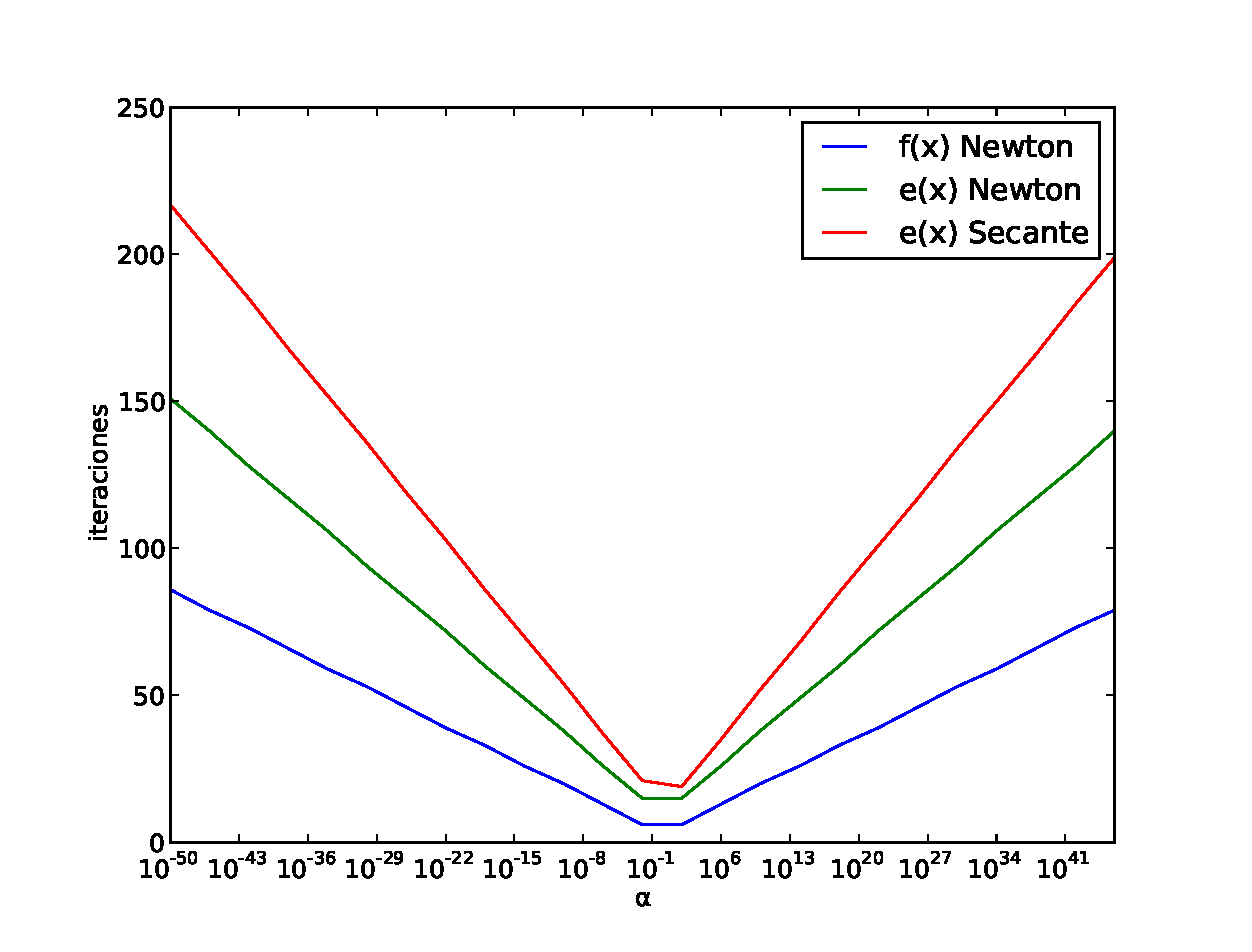
\includegraphics[scale=0.5]{graficos/new/comparacion_iteraciones.eps}
    \caption{\label{fig:comparacion_iteraciones} Gráfico comparativo de $\alpha$ en función de la cantidad de iteraciones}
  \end{center}
\end{figure}

Como podemos ver en la Figura~\ref{fig:comparacion_iteraciones} nuestras expectactivas se cumplieron, y podemos ver además como las iteraciones disminuyen a medida que los puntos iniciales están cerca del $\alpha$.

% subsubsection iteraciones (end)

\subsubsection{Tiempo de Ejecución} % (fold)
\label{ssub:tiempo_de_ejecuci_n}

Para hacer el cálculo del tiempo lo que hicimos fue hacer 1000 corridas de cada método y luego tomar el promedio, de esta manera podemos descartar outliers. En esta sección entra en juego lo que hablamos en la parte de Hipótesis. En términos prácticos, uno de los factores a tomar en cuenta es cuán rápido obtenemos el resultado requerido. Como bien enunciamos anteriormente suponemos que Secante será mas rápido que Newton.\\

\begin{figure}[!htbp]
  \begin{center}
    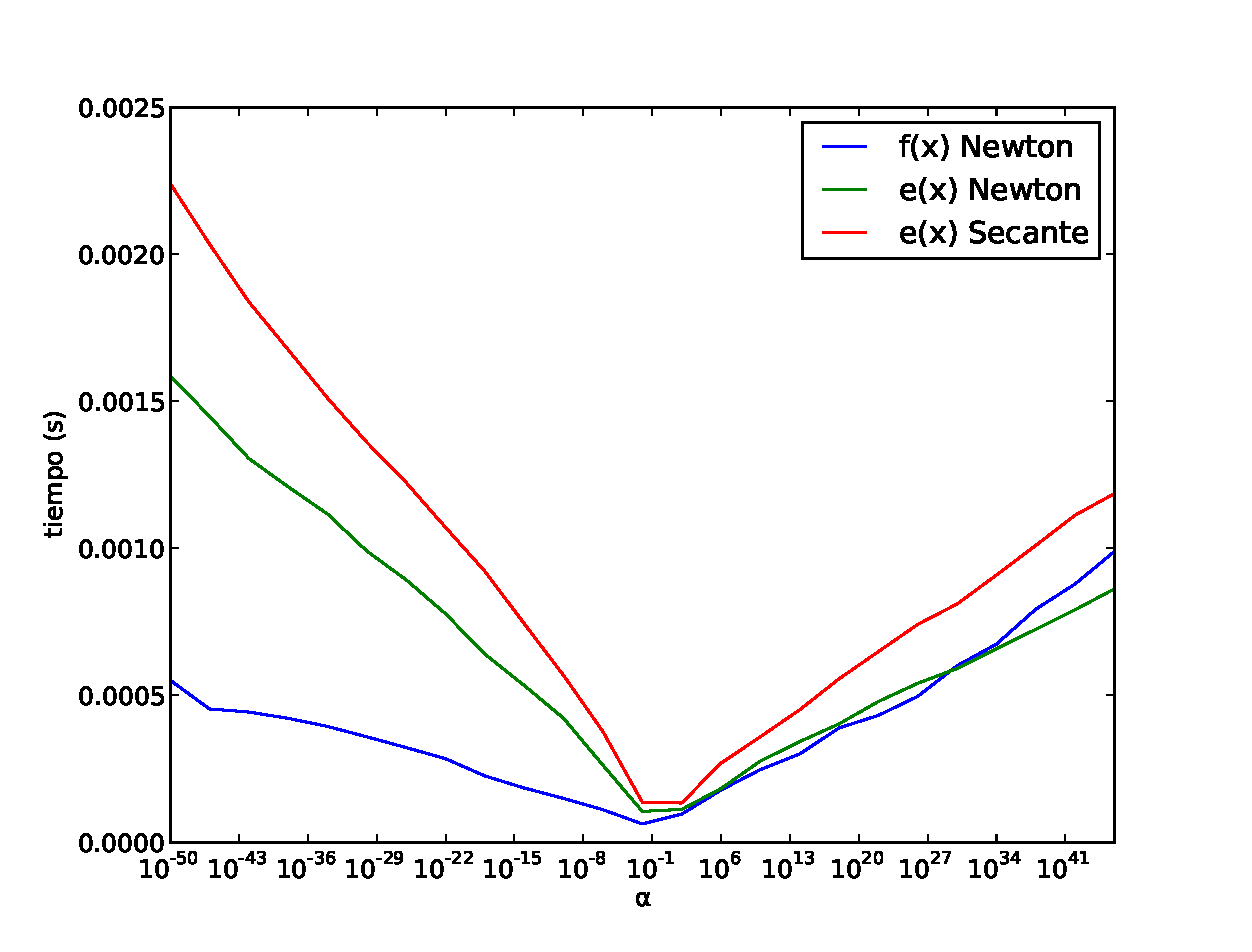
\includegraphics[scale=0.5]{graficos/new/comparacion_tiempos.eps}
    \caption{\label{fig:comparacion_tiempos} Gráfico comparativo de $\alpha$ en función del tiempo de ejecución}
  \end{center}
\end{figure}

En la Figura~\ref{fig:comparacion_tiempos} vemos cómo lo que habíamos anticipado al final no sucede, Newton con $f(x)$ es el que termina siendo mas performante y lo otro que podemos ver es que para $e(x)$ con Newton y Secante, el primero es mas performante desde valores chicos, pasando por el valor exacto, hasta que cuando $alpha$ crece mas, llega un punto donde Newton supera a Secante.\\

% subsubsection tiempo_de_ejecuci_n (end)